\begin{figure}[ht]
	\centering
	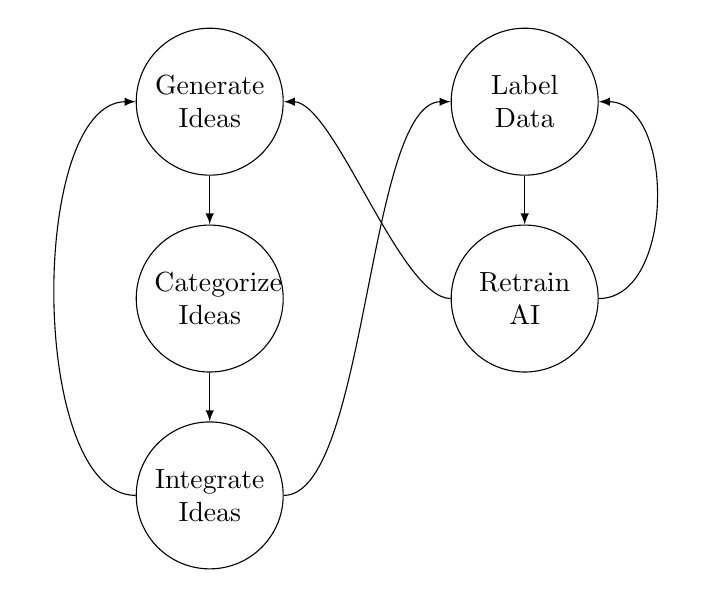
\begin{tikzpicture}[node distance=2.5cm, auto]
		% Styles
		\tikzset{
			block/.style={circle, draw, text width=4em, align=center, minimum height=3em},
			line/.style={draw, -latex} % Correct arrow tip style
		}
		
		% Nodes for the left vertical cycle
		\node[block] (1) {Generate Ideas};
		\node[block, below of=1] (2) {Categorize Ideas};
		\node[block, below of=2] (3) {Integrate Ideas};
		
		% Nodes for the right vertical cycle
		\node[block, right of=1, node distance=4cm] (4) {Label Data};
		\node[block, below of=4] (5) {Retrain AI};
		
		% Arrows for the left cycle
		\draw[line] (1) -- (2);
		\draw[line] (2) -- (3);
		\draw[line] (3) to[out=180, in=180, looseness=0.7] (1);  % Looping back from 3 to 1
		
		% Arrows for the right cycle
		\draw[line] (4) -- (5);
		\draw[line] (5) to[out=360, in=360, looseness=1] (4);  % Looping back from 5 to 4
		
		% Additional connections
		\draw[line] (5) to[out=180, in=360, looseness=0.5] (1);
		\draw[line] (3) to[out=360, in=180, looseness=0.5] (4);
		
	\end{tikzpicture}
	\caption{Schematic Representation of Two Interconnected Cycles}
	\label{fig:cycles}
\end{figure}